\documentclass{homework}
\usepackage{lipsum}
\usepackage{cancel}
\usepackage{amsthm}
\usepackage{cleveref}
\usepackage{upgreek}
\usepackage{mathrsfs}
\usepackage{tikz}
\usepackage{units}
\usepackage{slashbox}
\newtheorem{lemma}{Lemma}

\DeclareMathOperator{\cov}{cov}

\title{Kevin Joyce}
\course{Stat 542 - Applied Linear Models - Homework 6}
\author{Kevin Joyce}
\docdate{\today}
\begin{document} 
\newcommand{\figref}[1]{\figurename~\ref{#1}}
\renewcommand{\bar}{\overline}
\renewcommand{\hat}{\widehat}
\renewcommand{\SS}{\mathcal S}
\newcommand{\HH}{\mathscr H}
\newcommand{\mom}{\widetilde}
\newcommand{\mle}{\widehat \Uptheta}
\newcommand{\eps}{\varepsilon}
\newcommand{\todist}{\stackrel{D}\longrightarrow}
\newcommand{\toprob}{\stackrel{p}\longrightarrow}
\newcommand{\TTheta}{\overline{\underline \Theta} }
\newcommand{\del}{\partial}
\newcommand{\approxsim}{\overset{\cdotp}{\underset{\cdotp}{\sim}}}
\newcommand{\RSS}{\ensuremath{\mathrm{RSS}}}
\newcommand{\MSE}{\ensuremath{\mathrm{MSE}}}
\newcommand{\SE}{\ensuremath{\mathrm{SE}}}
\newcommand{\TSS}{\ensuremath{\mathrm{TSS}}}
\newcommand{\SSReg}{\ensuremath{\mathrm{SSReg}}}
\renewcommand{\a}[1]{{\color{red} \it #1}}

\problem{Analyze \texttt{warpbreaks} data as a two-way ANOVA.  Which factors are significant?  Now check for a good transformation on the response and see wheter the model may be simplified.  Now form a six-level factor from all combinations of the \texttt{wool} and \texttt{tension} factors.  Which combinations are significantly different?}

\begin{solution}
\begin{minipage}{.5\textwidth}
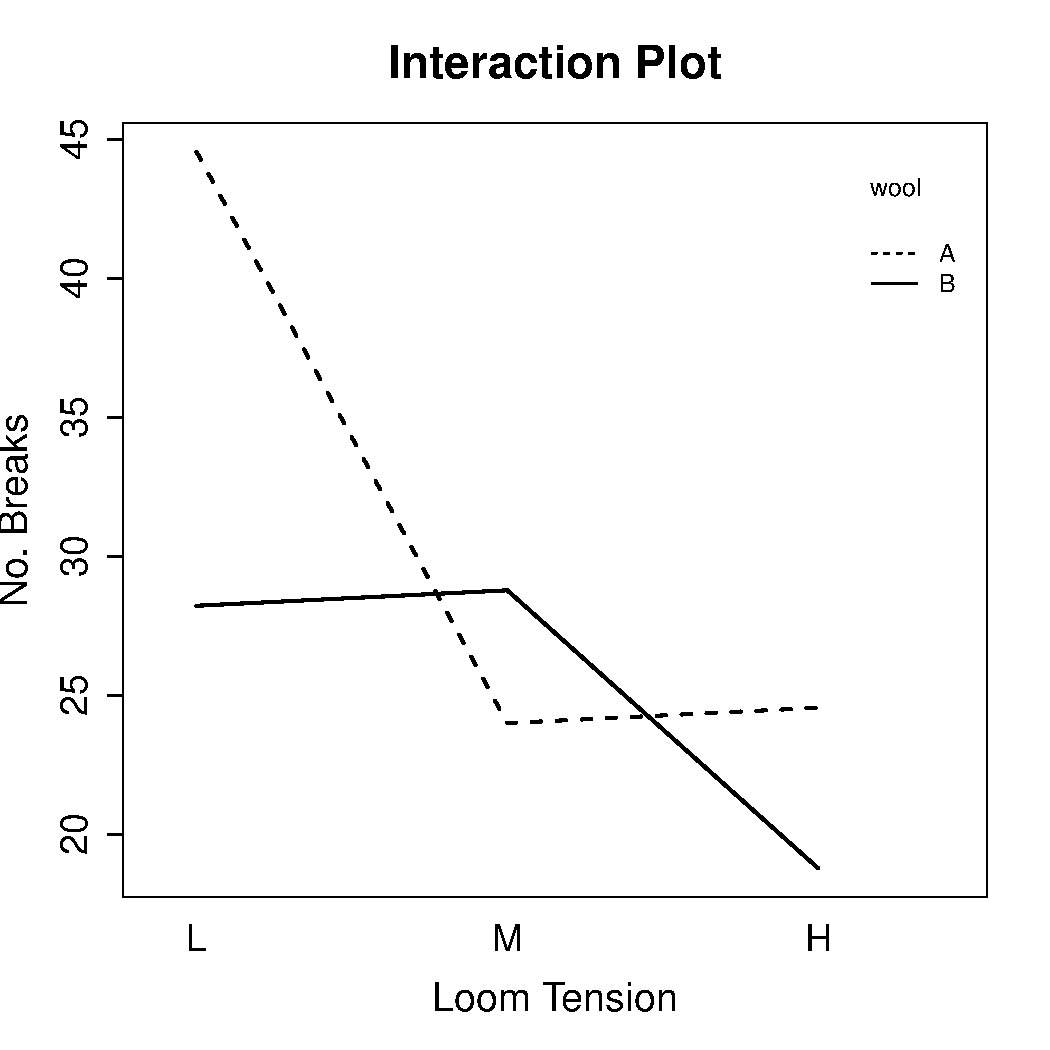
\includegraphics[width=\textwidth]{wool_interaction1.pdf}
\end{minipage}
\begin{minipage}{.5\textwidth}
The interaction plot to the left suggests that an interaction may be significant between the wool type and loom tension in modeling the number of breaks. Indeed, when we fit a two way ANOVA model, the interaction term is found to be moderately significant ($p=0.021$). 
{\small
\begin{verbatim}
Response: breaks
             Df Sum Sq Mean Sq F value    Pr(>F)    
tension       2 2034.3 1017.13  8.4980 0.0006926 ***
wool          1  450.7  450.67  3.7653 0.0582130 .  
tension:wool  2 1002.8  501.39  4.1891 0.0210442 *  
Residuals    48 5745.1  119.69                      
\end{verbatim}
}
\end{minipage}

Although, checking the model assumptions, provides evidence of
variance heterogeneity.  It appears that there is higher variance for
configurations that lead to more breaks.  Applying a log
transformation seems to mitigate this problem.
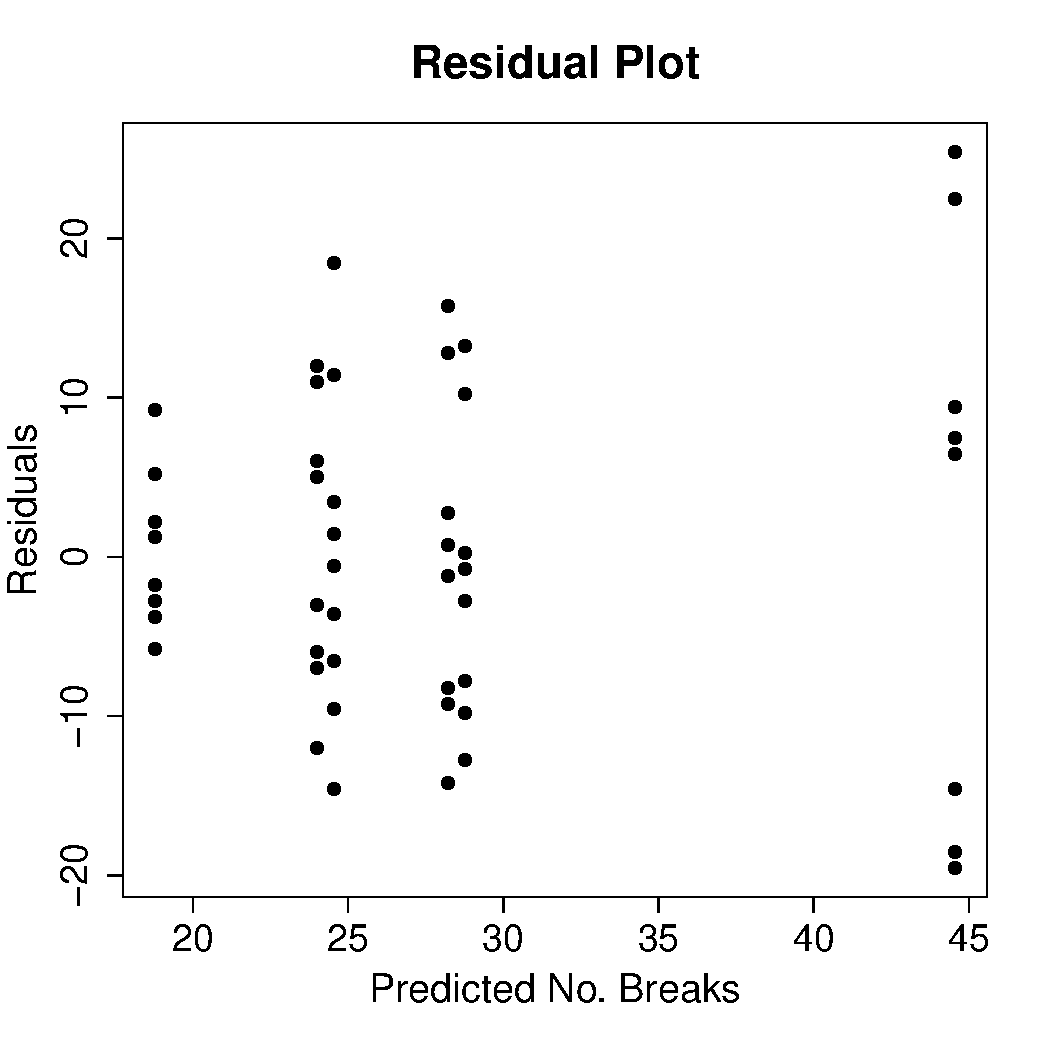
\includegraphics[width=.45\textwidth]{wool_resid1.pdf}
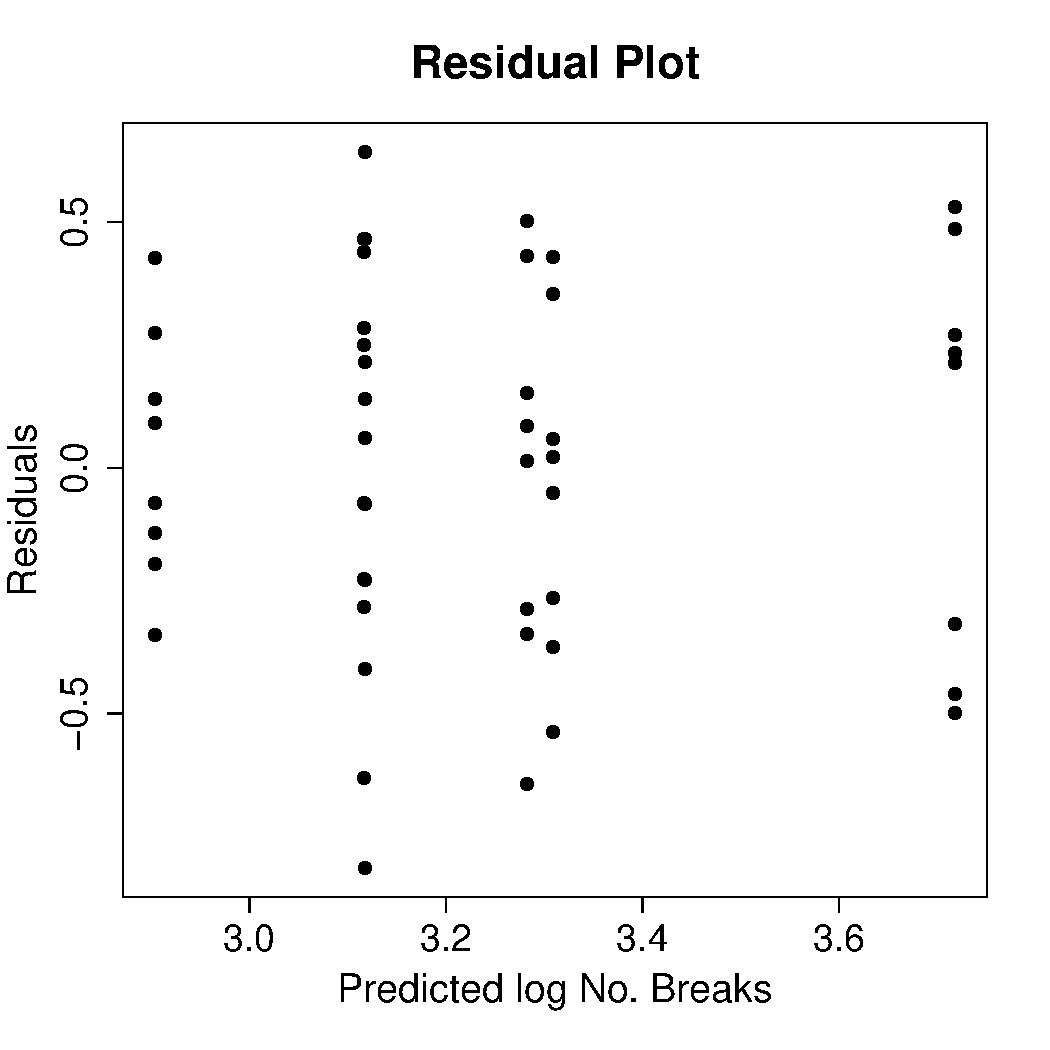
\includegraphics[width=.45\textwidth]{wool_resid2.pdf}

\begin{minipage}{.5\textwidth}
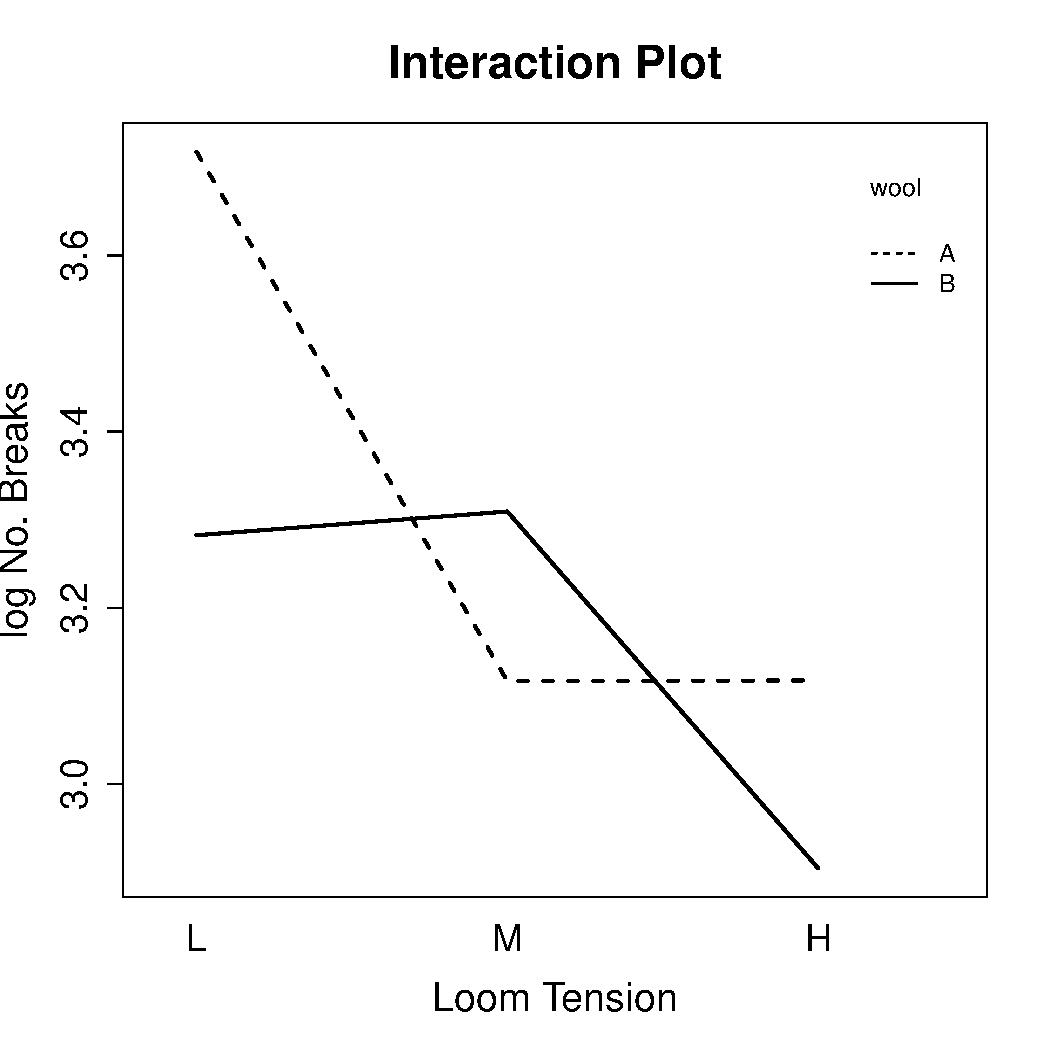
\includegraphics[width=\textwidth]{wool_interaction3.pdf}
\end{minipage}
\begin{minipage}{.5\textwidth}
  There still appears to be an interaction between tension and wool
  type, and the two way ANOVA provides moderate statistcal evidence
  of this ($p=0.047$).  Hence, further analysis of effects must be done within each factor level.
{\small
\begin{verbatim}
Response: log(breaks)
             Df Sum Sq Mean Sq F value   Pr(>F)   
tension       2 2.1762 1.08808  7.7792 0.001185 **
wool          1 0.3125 0.31253  2.2344 0.141511   
tension:wool  2 0.9131 0.45657  3.2642 0.046863 * 
Residuals    48 6.7138 0.13987                    
\end{verbatim}
}
\end{minipage}
\end{solution}

\begin{longproblem}
  The \texttt{eggprod} dataset in the \texttt{faraway} library concerns an experiment where six pullets were placed into each of 12 pens.  Four blocks were formed from groups of three pens based on location.  Three treatments were applied.  The number of eggs produced was recorded.

  \subproblem{ Fit a model for the number of eggs produced with the treatments as fixed effects and the blocks as random effects.  Describe the estimated differences between the treatments.}

  \subproblem{ Test for the significance of the treatment.  Compute the p-value using both the $\chi^2$-distribution (with a likelihood ratio test) and resampling methods (bootstrapping). }
\end{longproblem}
\end{document} 

